
\chapter{Analysis}

\section{Performance}

\begin{figure}[h!]
    \centering
    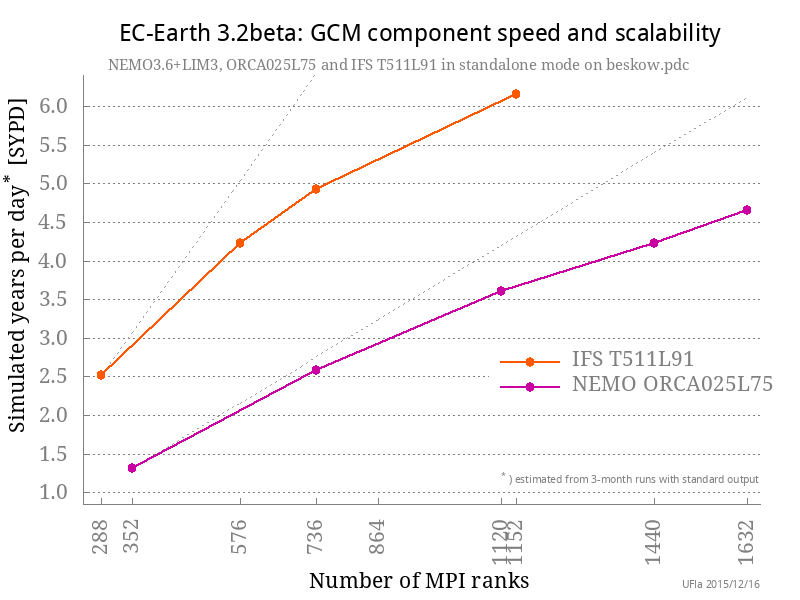
\includegraphics[scale=0.4]{figs/ece32b-speedup}
    \caption{HiRes IFS and NEMO speedup}
    \label{fig:hires-speed}
\end{figure}

Figure~\ref{fig:hires-speed} plots the tests for NEMO and IFS in highres mode by Uwe Fladrich. Note that
this is not coupled, one has to allow for some coupling overhead for the final model.

\begin{table}
\begin{tabular}{|l|c|c|c|}
    \hline
    Parameter& T159-ORCA1& T255-ORCA1& T799-ORCA0.25\\
    \hline
    IFS timestep& 1 hour& 1 hour& 12 minutes\\
    IFS input file size& 29MB& 95MB& 680MB\\
    IFS 2D grid snapshot size& 12MB& 16.5MB& 107MB\\
    IFS \#2D snapshots& 161& 63& 63\\
    IFS spectral snapshot size& 13MB& 6MB& 67MB\\
    IFS snapshot frequency& 6 hourly& 6 hourly& 6 hourly\\
    NEMO timestep& 1 hour& 1 hour& 20 minutes\\
    NEMO output freq.& varying& varying& varying\\
    LIM2 timestep& 1 hour& 1 hour& 1 hour\\
    OASIS coupling freq.& 3 hours& 3 hours& 3 hours    \\
    \hline 
\end{tabular}
\caption{Parameters of different EC-EARTH configurations}%TODO: update}
\end{table}

For more details on the performance of NEMO, we refer to the BSC technical report~\cite{nemo-per15}. More simulation results are 
available at~\cite{ece-sim,prace12}.

\section{Profiling}
\section{Callgraph}

\section{Future steps}
\begin{itemize}
    \item Possible extension to other domains
    \item Diff between main svn branch and HiRes branch for the future easy merge
\end{itemize}

